\documentclass[11pt]{article}

\usepackage[margin=1in]{geometry}
\usepackage{amsmath,amssymb,amsfonts,amsthm}
\usepackage{graphicx}
\usepackage{booktabs}
\usepackage{hyperref}
\usepackage[numbers,sort&compress]{natbib}
\usepackage{microtype}

\graphicspath{{../cycle_moment_outputs/}}

\newtheorem{theorem}{Theorem}
\newtheorem{lemma}{Lemma}
\newtheorem{proposition}{Proposition}
\newtheorem{remark}{Remark}

\newcommand{\B}{\mathcal B}
\newcommand{\one}{\mathbf 1}
\newcommand{\tr}{\operatorname{tr}}
\newcommand{\grad}{\operatorname{grad}}
\newcommand{\diag}{\operatorname{diag}}
\newcommand{\R}{\mathbb R}

\title{Cycle-Moment Sinkhorn Flows:\\A Brockett-like View of Trace-Constrained Routing on the Birkhoff Polytope}
\author{Paul Bellette}
\date{Draft: \today}

\begin{document}
\maketitle

\begin{abstract}
We sketch a geometric flow on the positive interior of the Birkhoff polytope motivated by the traveling salesperson problem, Brockett's double-bracket flow, and modern Sinkhorn and mirror-descent methods. The central object is a KL-gradient flow over doubly stochastic matrices augmented by trace-power constraints of the form
\[
    h_k(P)=\tr(P^k)-b_k.
\]
For TSP-like routing, these trace moments distinguish single Hamiltonian cycles from subtour decompositions. The resulting system is not proposed primarily as a competitive TSP solver, but as a mathematical object: a transport-polytope analogue of Brockett-style constrained matrix flows. We discuss its constrained geometry, primal-dual and augmented variants, local linearisation, Lyapunov structure, damping of trace-violating modes, degeneracy near the uniform doubly stochastic matrix, and reduced-cost stability near permutation vertices. Small numerical experiments illustrate the predicted stability phenomena.
\end{abstract}

\section{Motivation}

Brockett's double-bracket flow gives a dynamical-systems view of sorting, diagonalisation, and constrained matrix evolution \citep{brockett1991dynamical}. Classical Brockett-style flows usually live on isospectral or orthogonal/conjugacy manifolds, where commutator structure preserves constraints while a potential function drives the system toward an ordered state.

Here we ask for an analogous object on the Birkhoff polytope
\[
    \B_n=\{P\in\R_+^{n\times n}:P\one=\one,\;P^\top\one=\one\}.
\]
The vertices of $\B_n$ are permutation matrices by the Birkhoff--von Neumann theorem. For directed TSP, a tour can be represented by a permutation matrix corresponding to a single $n$-cycle. The usual assignment relaxation allows all permutation matrices, including disjoint subtour decompositions. Trace powers provide a compact differentiable way to detect closed walks and subtours.

The motivating question is:
\begin{quote}
Can we define a Brockett-like flow on the Birkhoff polytope whose geometry is Sinkhorn/KL rather than orthogonal/commutator, and whose moment constraints favour Hamiltonian cycles?
\end{quote}
The practical version is a differentiable Sinkhorn relaxation for TSP. The more interesting mathematical version is a constrained mirror-gradient flow with trace moments and a stability theory that may apply more generally to differentiable routing and assignment problems.

\section{Birkhoff and trace-moment setup}

Let $P\in\B_n^\circ$, where
\[
    \B_n^\circ=\{P>0:P\one=\one,\;P^\top\one=\one\}.
\]
Let $C\in\R^{n\times n}$ be an edge-cost matrix. The linear assignment/TSP-like cost is
\[
    \langle C,P\rangle=\tr(C^\top P).
\]
Define trace-moment constraints
\[
    h_k(P)=\tr(P^k)-b_k.
\]
For a single directed Hamiltonian cycle, a natural target is
\[
    b_k=0,\quad 1\le k<n,\qquad b_n=n.
\]
The constraints $\tr(P^k)=0$ for $k<n$ suppress shorter closed cycles, while $\tr(P^n)=n$ is consistent with a single $n$-cycle permutation. Trace powers and related trace/exponential trace constraints are common in continuous acyclicity formulations \citep{zheng2018dags}; recent work has also explored trace-guided continuous relaxations for ATSP \citep{zhang2026solving}.

\begin{lemma}[Trace moments characterise Hamiltonian cycles]
Let $P\in\B_n$. Then $P$ is the permutation matrix of a single directed $n$-cycle if and only if
\[
    \tr(P^k)=0,\qquad k=1,\dots,n-1.
\]
In that case, automatically $\tr(P^n)=n$.
\end{lemma}

\begin{proof}
If $P$ is a single $n$-cycle permutation matrix, then $P^k$ has no fixed points for $1\le k<n$, so $\tr(P^k)=0$.

Conversely, suppose $P\in\B_n$ and $\tr(P^k)=0$ for $1\le k<n$. Since $P\ge0$,
\[
    \tr(P^k)=\sum_{i_1,\ldots,i_k}P_{i_1i_2}P_{i_2i_3}\cdots P_{i_ki_1},
\]
and every term is nonnegative. Hence $\tr(P^k)=0$ implies there is no positive-weight closed walk of length $k$.

By the Birkhoff--von Neumann theorem, write
\[
    P=\sum_\ell \alpha_\ell \Pi_\ell,\qquad \alpha_\ell>0,\quad \sum_\ell\alpha_\ell=1,
\]
where each $\Pi_\ell$ is a permutation matrix. If any $\Pi_\ell$ contained a cycle of length $m<n$, that cycle would give a positive term in $\tr(P^m)$, a contradiction. Hence each $\Pi_\ell$ is a single $n$-cycle.

It remains to rule out a convex combination of distinct $n$-cycles. Relabel the vertices so that one such cycle is
\[
    1\to2\to\cdots\to n\to1.
\]
If another $n$-cycle is distinct, it has some edge $i\to j$ with $j\ne i+1$ modulo $n$. Combining this edge with the path in the first cycle from $j$ back to $i$ gives a directed cycle of length strictly less than $n$ in the support of $P$, again contradicting the trace constraints. Therefore all permutation matrices in the decomposition are the same $n$-cycle, and $P$ is that permutation matrix. Finally $P^n=I$, so $\tr(P^n)=n$.
\end{proof}

\begin{remark}
On an orthogonal or isospectral manifold, trace-power constraints mostly constrain eigenvalues and leave a large continuous orbit. On the nonnegative stochastic/Birkhoff side, trace powers have a direct closed-walk interpretation. This is what makes the trace constraints combinatorial.
\end{remark}

\section{KL geometry on the Birkhoff polytope}

A natural flow on $\B_n^\circ$ is the KL or entropic mirror-gradient flow. Given a scalar energy $E(P)$ with Euclidean gradient $G=\nabla_P E(P)$, the Birkhoff-preserving mirror flow can be written
\[
    \dot P_{ij}=-P_{ij}(G_{ij}-a_i-b_j),
\]
where row and column potentials $a,b$ are chosen so that $\dot P\one=0$ and $\dot P^\top\one=0$. This is related to Sinkhorn and mirror-flow viewpoints on transport polytopes \citep{karimi2023sinkhorn,ballu2023mirror,nutz2021introduction}.

Let
\[
    r_i=\sum_jP_{ij}G_{ij},\qquad c_j=\sum_iP_{ij}G_{ij}.
\]
Preservation of row and column sums gives
\[
    a+Pb=r,
\]
\[
    P^\top a+b=c,
\]
or
\[
\begin{bmatrix} I&P\\ P^\top&I\end{bmatrix}
\begin{bmatrix} a\\ b\end{bmatrix}
=
\begin{bmatrix} r\\ c\end{bmatrix}.
\]
There is a gauge freedom $a\mapsto a+\gamma\one$, $b\mapsto b-\gamma\one$.

The tangent space of the Birkhoff interior is
\[
    T_P\B_n^\circ=\{V\in\R^{n\times n}:V\one=0,\;V^\top\one=0\}.
\]
The KL/Fisher metric on positive matrices is
\[
    \langle U,V\rangle_P=\sum_{ij}\frac{U_{ij}V_{ij}}{P_{ij}}.
\]
Without row/column constraints, the KL-gradient of $E$ is $P\odot G$, because
\[
    \langle P\odot G,V\rangle_P=\sum_{ij}G_{ij}V_{ij}=DE(P)[V].
\]
The Birkhoff constraints subtract row and column potentials before multiplying by $P$.

Define
\[
    W_{ij}=P_{ij}(G_{ij}-a_i-b_j).
\]
For any tangent direction $V\in T_P\B_n^\circ$,
\begin{align*}
    \langle W,V\rangle_P
    &=\sum_{ij}(G_{ij}-a_i-b_j)V_{ij}\\
    &=\sum_{ij}G_{ij}V_{ij}
      -\sum_i a_i\sum_jV_{ij}
      -\sum_j b_j\sum_iV_{ij}\\
    &=DE(P)[V].
\end{align*}
The potential terms vanish because tangent directions have zero row and column sums. Hence $W=\grad^{\mathrm{KL}}_{\B}E(P)$, and the negative KL-gradient flow is $\dot P=-W$.

Strict positivity follows from the multiplicative form. Each entry satisfies $\dot P_{ij}=P_{ij}R_{ij}(t)$, so
\[
    P_{ij}(t)=P_{ij}(0)\exp\left(\int_0^tR_{ij}(s)\,ds\right),
\]
and positive entries remain positive while the vector field remains finite.

\section{Cycle-moment Sinkhorn flow}

Define the augmented trace-penalty energy
\[
    E_\rho(P)=\langle C,P\rangle+\frac{\rho}{2}\sum_{k=1}^nh_k(P)^2.
\]
Then
\[
    \nabla_P E_\rho(P)=C+\rho\sum_{k=1}^n h_k(P)\,k(P^{k-1})^\top.
\]
The penalty flow is therefore
\[
    \dot P_{ij}=-P_{ij}(G_{ij}-a_i-b_j).
\]
This is the continuous-time analogue of exponentiated-gradient descent followed by Sinkhorn projection.

\section{Trace derivatives and constraint Jacobian}

Let $f_k(P)=\tr(P^k)$. Expanding to first order,
\[
    (P+\epsilon\delta P)^k=P^k+\epsilon\sum_{r=0}^{k-1}P^r\delta P P^{k-1-r}+O(\epsilon^2).
\]
Taking traces and using cyclicity gives
\[
    Df_k(P)[\delta P]=k\tr(P^{k-1}\delta P).
\]
Thus
\[
    \nabla_P\tr(P^k)=k(P^{k-1})^\top.
\]
The trace-constraint Jacobian $A=Dh(P)$ has rows
\[
    A_k[\delta P]=k\tr(P^{k-1}\delta P).
\]
Differentiating again gives the directional second variation
\[
    D^2f_k(P)[\delta P,\delta P]
    =k\sum_{r=0}^{k-2}\tr(P^r\delta P P^{k-2-r}\delta P).
\]
The linear cost contributes no Hessian; local curvature of the trace-constrained Lagrangian is generated by the trace terms.

\section{Primal-dual and augmented variants}

Introduce live multipliers $\lambda_k$ and define
\[
    \mathcal L(P,\lambda)=\langle C,P\rangle+\sum_{k=1}^n\lambda_kh_k(P).
\]
The primal-dual mirror flow is
\[
    \dot P=-\grad^{\mathrm{KL}}_\B\mathcal L(P,\lambda),\qquad \dot\lambda_k=\eta h_k(P).
\]
The augmented version is
\[
    \mathcal L_\rho(P,\lambda)=\langle C,P\rangle+\lambda^\top h(P)+\frac{\rho}{2}\|h(P)\|^2.
\]
The augmented term is not merely a penalty; locally it damps trace-visible primal-dual modes, as described below.

\section{Lyapunov structure}

For any smooth energy $E$ and KL-gradient flow $\dot P=-W$, where $W=\grad^{\mathrm{KL}}_\B E(P)$,
\[
    \frac{dE}{dt}=DE(P)[\dot P]=\langle W,-W\rangle_P=-\|W\|_P^2\le0.
\]
In coordinates,
\[
    \|W\|_P^2=\sum_{ij}P_{ij}(G_{ij}-a_i-b_j)^2.
\]
Thus for the pure penalty flow,
\[
    \frac{dE_\rho}{dt}=-\sum_{ij}P_{ij}(G_{ij}-a_i-b_j)^2\le0.
\]
The pure primal-dual flow does not satisfy the same identity for $\mathcal L$. Indeed,
\[
    \frac{d\mathcal L}{dt}=D_P\mathcal L[\dot P]+h(P)^\top\dot\lambda,
\]
and with $\dot\lambda=\eta h(P)$ the second term is $\eta\|h(P)\|^2\ge0$. This is consistent with the oscillatory modes of the primal-dual linearisation.

\section{Local linearisation and damping}

Let $(P_*,\lambda_*)$ be an interior stationary point and let $A_*=Dh(P_*)$. Schematically, the primal-dual linearisation has block form
\[
\begin{bmatrix}
\delta\dot P\\
\delta\dot\lambda
\end{bmatrix}
=
\begin{bmatrix}
-M_*H_*&-M_*A_*^\top\\
\eta A_*&0
\end{bmatrix}
\begin{bmatrix}
\delta P\\
\delta\lambda
\end{bmatrix}.
\]
Here $M_*$ denotes the KL mobility/projection operator at $P_*$. Concretely, for a Euclidean covector $Q$, $M_*Q$ is the Birkhoff-tangent vector
\[
    (M_*Q)_{ij}=P_{*,ij}(Q_{ij}-\alpha_i-\beta_j),
\]
where $\alpha,\beta$ are chosen so that $M_*Q$ has zero row and column sums.

For the augmented primal-dual flow, the schematic linearisation becomes
\[
\begin{bmatrix}
\delta\dot P\\
\delta\dot\lambda
\end{bmatrix}
=
\begin{bmatrix}
-M_*(H_*+\rho A_*^\top A_*)&-M_*A_*^\top\\
\eta A_*&0
\end{bmatrix}
\begin{bmatrix}
\delta P\\
\delta\lambda
\end{bmatrix},
\]
with the caveat that the intrinsic metric-aware expression involves $M_*$, for example through $A_*M_*A_*^\top$ in the dual trace space.

For the clean trace-mode picture, use local coordinates $z$ on the Birkhoff tangent space and linearise $h(P_*+z)\approx Az$. Ignoring cost curvature, the pure primal-dual local model is
\[
    \dot z=-A^\top\lambda,
    \qquad
    \dot\lambda=\eta A z.
\]
Let $Av_i=\sigma_i u_i$ be a singular mode and write $z=qv_i$, $\lambda=pu_i$. Then
\[
    \dot q=-\sigma_i p,
    \qquad
    \dot p=\eta\sigma_i q,
\]
so
\[
    \ddot q+\eta\sigma_i^2q=0.
\]
This is the linearised ringing mechanism.

For the augmented system,
\[
    \dot z=-A^\top\lambda-\rho A^\top A z,
    \qquad
    \dot\lambda=\eta A z.
\]
The same singular mode satisfies
\[
    \ddot q+\rho\sigma_i^2\dot q+\eta\sigma_i^2q=0.
\]
Thus augmentation adds damping coefficient $\rho\sigma_i^2$ in each trace-visible singular mode. In the full nonlinear Sinkhorn parameterisation this undamped control structure may appear not as a clean sinusoid, but as delayed high-residual plateaus followed by sharp support changes.

\section{Uniform initialisation degeneracy}

Let
\[
    P_0=\frac{1}{n}\one\one^\top.
\]
Then $P_0^k=P_0$ for $k\ge1$. For $\delta P\in T_{P_0}\B_n$, and $k\ge2$,
\[
D\tr(P^k)|_{P=P_0}[\delta P]
=k\tr(P_0\delta P)
=\frac{k}{n}\one^\top\delta P\one=0.
\]
Thus all trace-power constraints with $k\ge2$ are first-order invisible at the uniform Birkhoff point. The case $k=1$ is special:
\[
    D\tr(P)[\delta P]=\tr(\delta P),
\]
which is not automatically zero on the Birkhoff tangent space. If diagonal/self-loop entries are hard-masked, this remaining first-order signal is removed. Consequently, in the no-self-loop setting, exact uniform initialisation is degenerate for trace penalties; small random logit perturbations are needed to reveal trace-gradient information.

\section{Boundary behaviour and reduced costs}

Permutation tours lie on the boundary of $\B_n$. The KL flow degenerates at zeros: if $P_{ij}=0$, then $\dot P_{ij}=0$. Boundary behaviour is therefore best interpreted through near-boundary limits or log coordinates.

For any positive entry,
\[
    \frac{d}{dt}\log P_{ij}=-(G_{ij}-a_i-b_j).
\]
Define the reduced augmented cost
\[
    \Delta_{ij}=G_{ij}-a_i-b_j.
\]
Then
\[
    \frac{d}{dt}\log P_{ij}=-\Delta_{ij}.
\]
Near a permutation tour, off-support entries are small but positive if we remain in the Birkhoff interior. Positive reduced cost suppresses such an edge; negative reduced cost makes it grow.

A single off-support edge is not generally a feasible perturbation. Feasible perturbations of a permutation vertex preserve row and column sums and are generated by alternating-cycle exchange directions in the assignment polytope \citep{balinski1974assignment}. If $D$ is such a feasible exchange direction, then $D\one=0$ and $D^\top\one=0$. Consequently,
\[
    \langle\Delta,D\rangle
    =\sum_{ij}(G_{ij}-a_i-b_j)D_{ij}
    =\langle G,D\rangle,
\]
because the row/column potentials vanish on feasible directions. Hence a candidate tour is locally stable against a feasible exchange direction $D$ when
\[
    \langle G,D\rangle>0.
\]
This is a reduced-cost diagnostic in the sense of linear programming and assignment optimisation \citep{luenberger1984linear}, not a global optimality theorem.

\section{Practical autodiff/Sinkhorn recipe}

The practical differentiable relaxation uses logits $X$ and a temperature $\tau$:
\[
    P=\operatorname{Sinkhorn}(\exp(X/\tau)).
\]
Then optimise
\[
    E_{\rho,\tau}(X)=\langle C,P\rangle+\frac{\rho}{2}\sum_{k=1}^n h_k(P)^2.
\]
The stability analysis suggests:
\begin{enumerate}
    \item do not initialise exactly at $X=0$ in the no-self-loop setting;
    \item use small random logits to break symmetry;
    \item increase $\rho$ gradually so trace-visible modes are damped without making the system excessively stiff;
    \item decrease $\tau$ gradually to encourage collapse toward permutation vertices;
    \item monitor reduced costs $\Delta_{ij}=G_{ij}-a_i-b_j$ near convergence.
\end{enumerate}

\section{Numerical investigation}

The experiments are diagnostic rather than benchmark-oriented. They test whether the stability predictions appear in small controlled instances.

\subsection{Circle sanity check}

On points arranged on a circle, the continuation schedule recovers the expected geometric tour. A fixed penalty can produce a valid cycle with poor geometry, demonstrating the separation between validity and optimality.

\begin{figure}[ht]
\centering
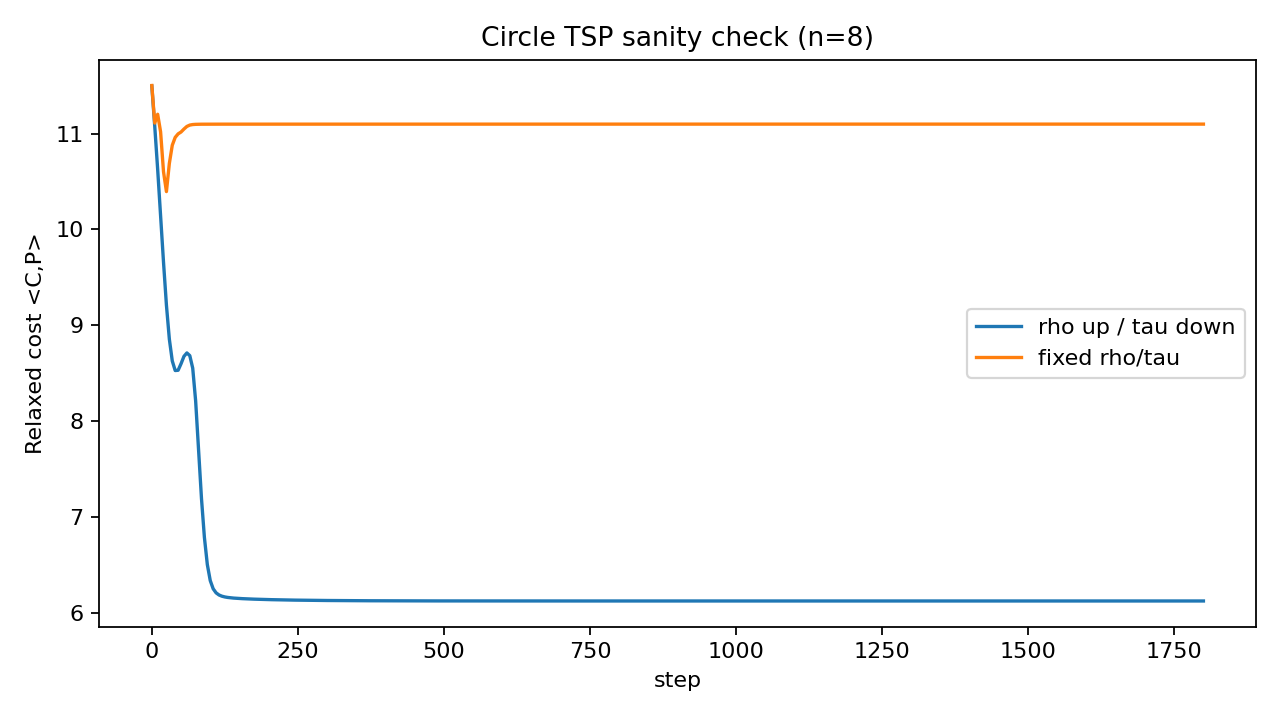
\includegraphics[width=.48\linewidth]{circle_cost.png}\hfill
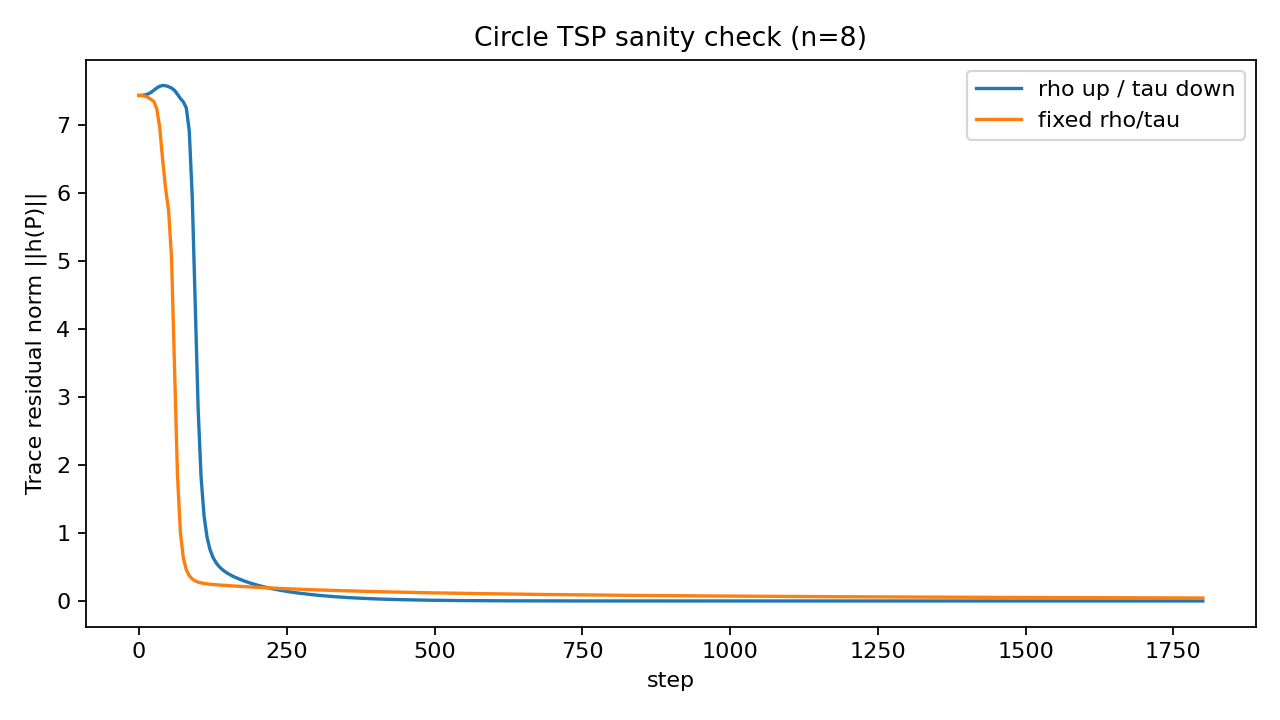
\includegraphics[width=.48\linewidth]{circle_h_norm.png}
\caption{Circle sanity check. The scheduled run reaches the optimal geometric tour cost while managing trace residuals.}
\label{fig:circle-diagnostics}
\end{figure}

\begin{figure}[ht]
\centering
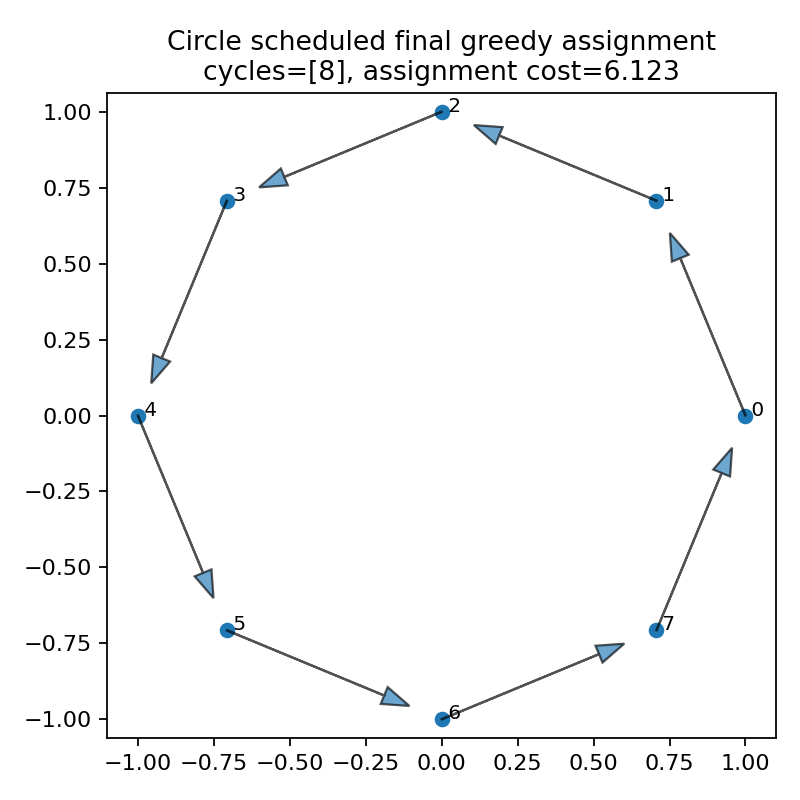
\includegraphics[width=.48\linewidth]{circle_scheduled_assignment_perm.png}\hfill
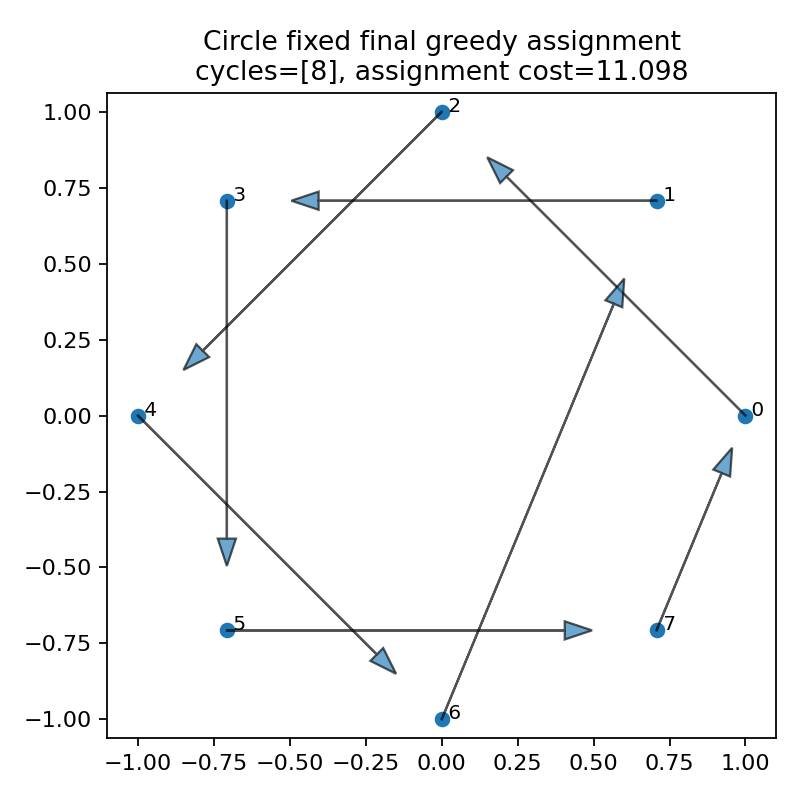
\includegraphics[width=.48\linewidth]{circle_fixed_assignment_perm.png}
\caption{Circle final assignments. The scheduled run recovers the nearest-neighbour tour; the fixed run can satisfy Hamiltonicity while selecting a poor crossing/chord tour.}
\label{fig:circle-assignments}
\end{figure}

\subsection{Two-cluster subtour pressure}

The two-cluster instance is designed so the cost favours two within-cluster subtours. Low trace pressure gives cheap cycle covers such as $[4,4]$; higher trace pressure forces a single 8-cycle.

\begin{figure}[ht]
\centering
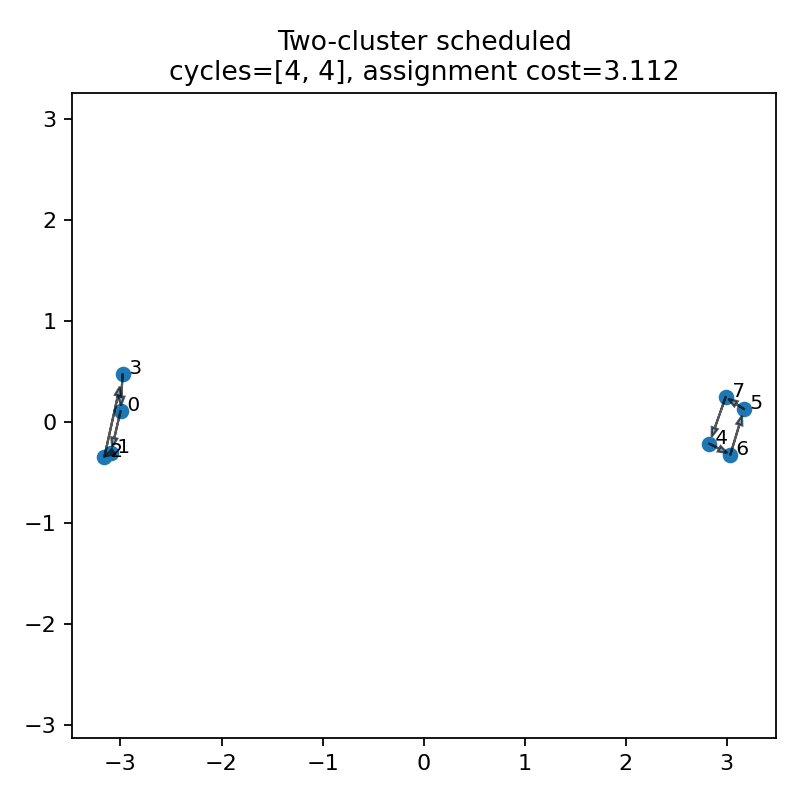
\includegraphics[width=.32\linewidth]{two_cluster_scheduled_assignment_perm.png}\hfill
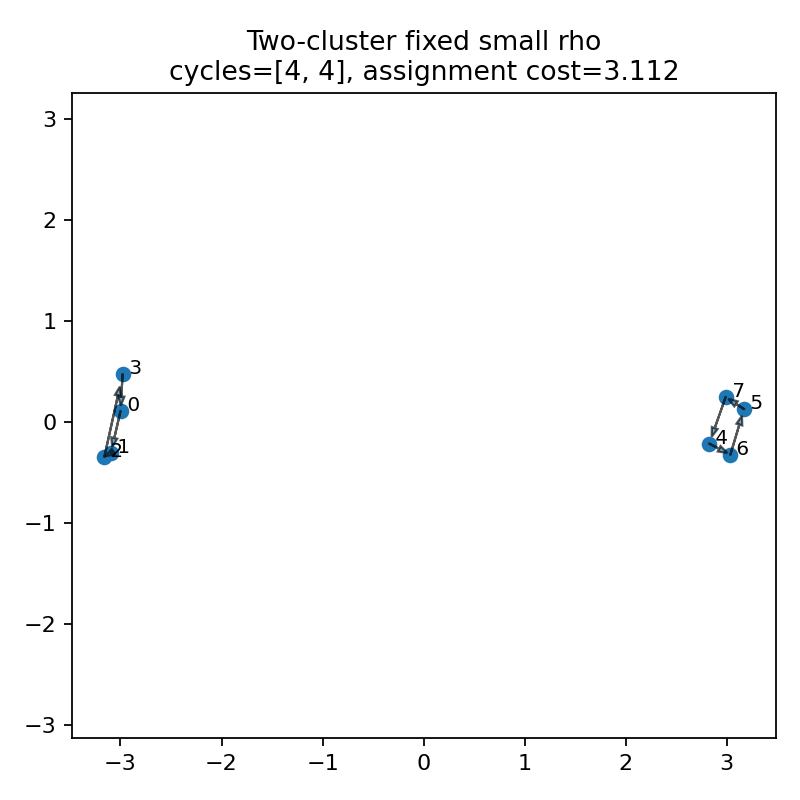
\includegraphics[width=.32\linewidth]{two_cluster_small_assignment_perm.png}\hfill
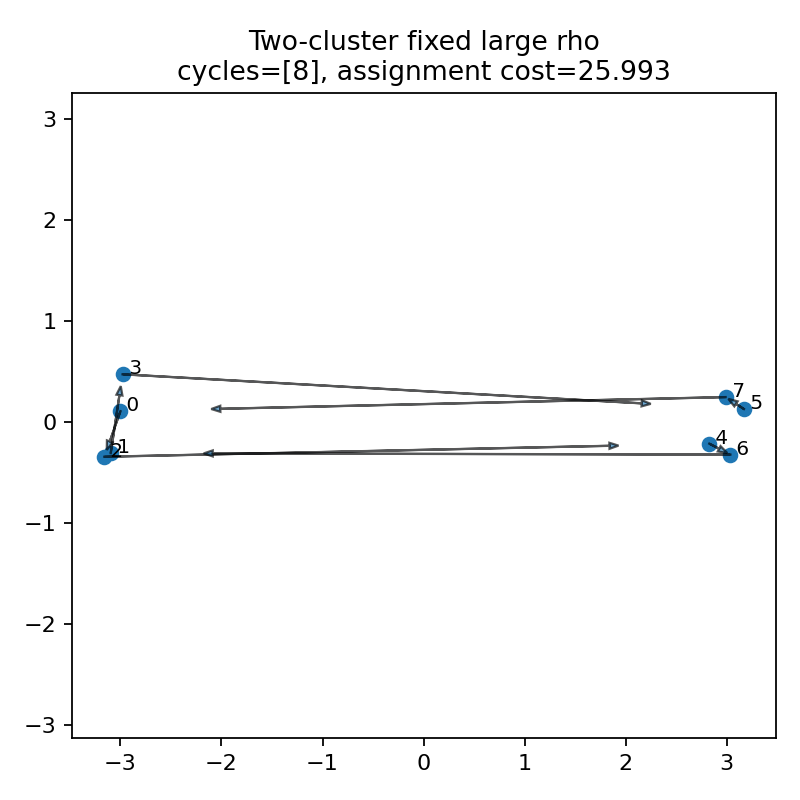
\includegraphics[width=.32\linewidth]{two_cluster_large_assignment_perm.png}
\caption{Two-cluster assignments. Scheduled and small-$\rho$ runs remain in subtour covers; large $\rho$ forces a single cycle.}
\label{fig:two-cluster-assignments}
\end{figure}

\subsection{Rho-pressure transition}

A fixed-$\rho$ sweep makes the Hamiltonicity-pressure transition explicit.

\begin{figure}[ht]
\centering
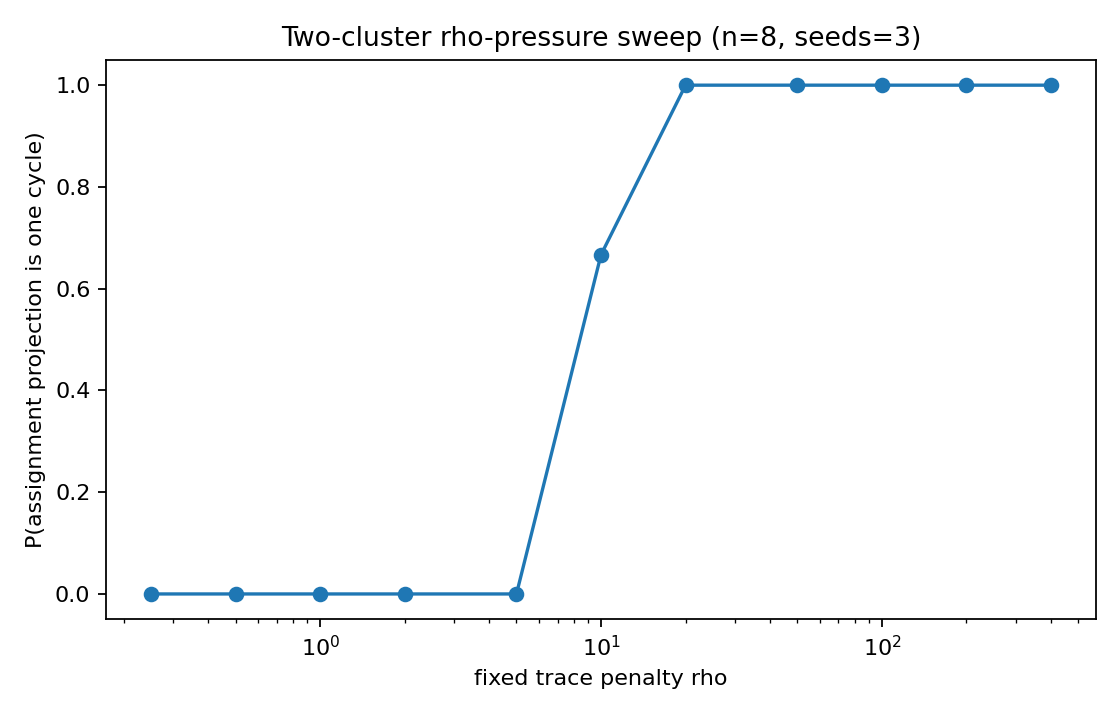
\includegraphics[width=.32\linewidth]{two_cluster_rho_pressure_single_cycle_probability.png}\hfill
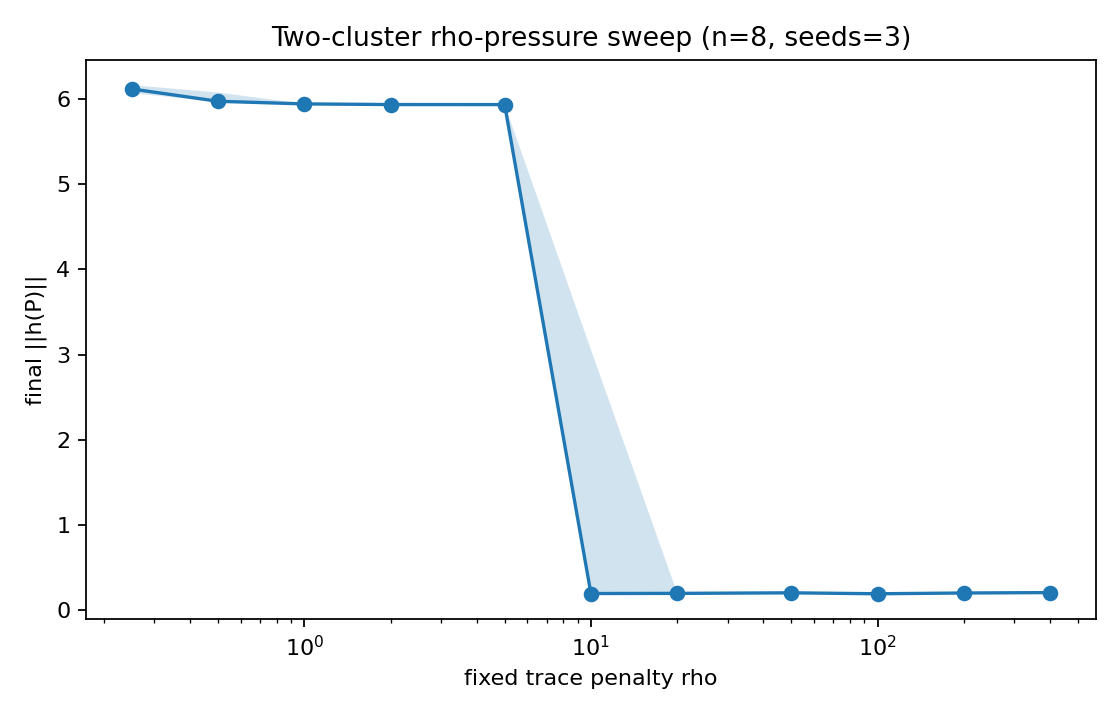
\includegraphics[width=.32\linewidth]{two_cluster_rho_pressure_h_norm_aggregate.png}\hfill
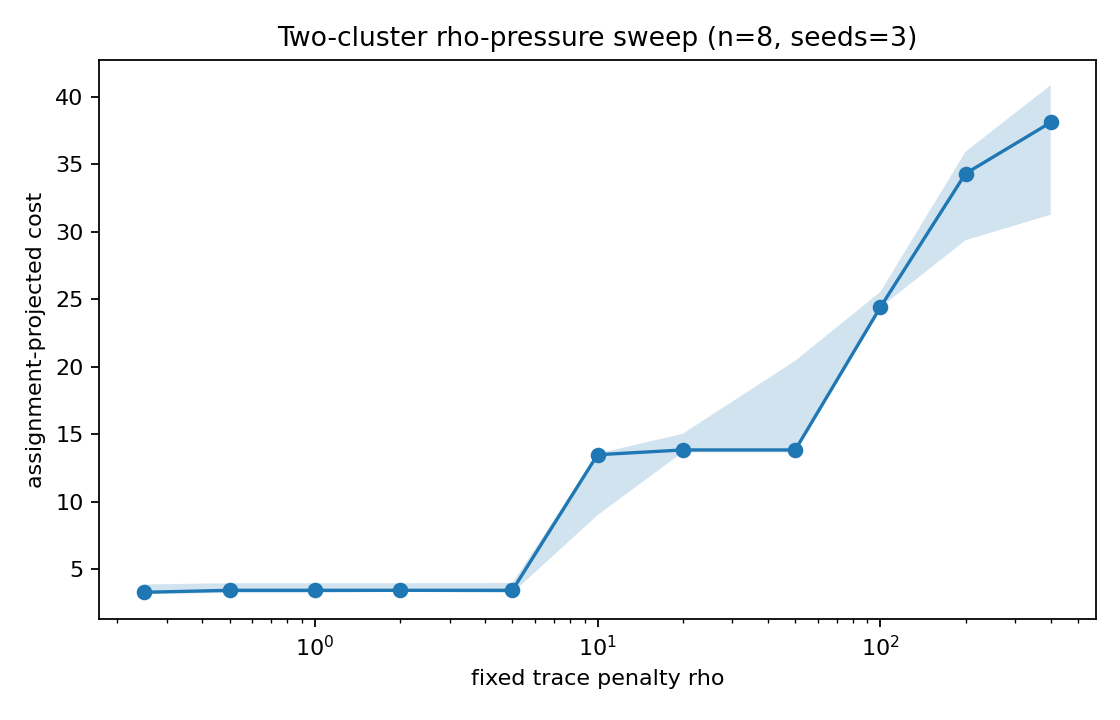
\includegraphics[width=.32\linewidth]{two_cluster_rho_pressure_assignment_cost_aggregate.png}
\caption{Rho-pressure sweep. Increasing $\rho$ collapses trace residuals and turns subtour covers into single-cycle assignments, but assignment-projected cost rises once Hamiltonicity is forced.}
\label{fig:rho-pressure}
\end{figure}

\subsection{Rho/tau phase diagram}

The phase diagram shows that $\rho$ primarily controls the subtour-to-Hamiltonian transition, while $\tau$ controls entropy and sharpness.

\begin{figure}[ht]
\centering
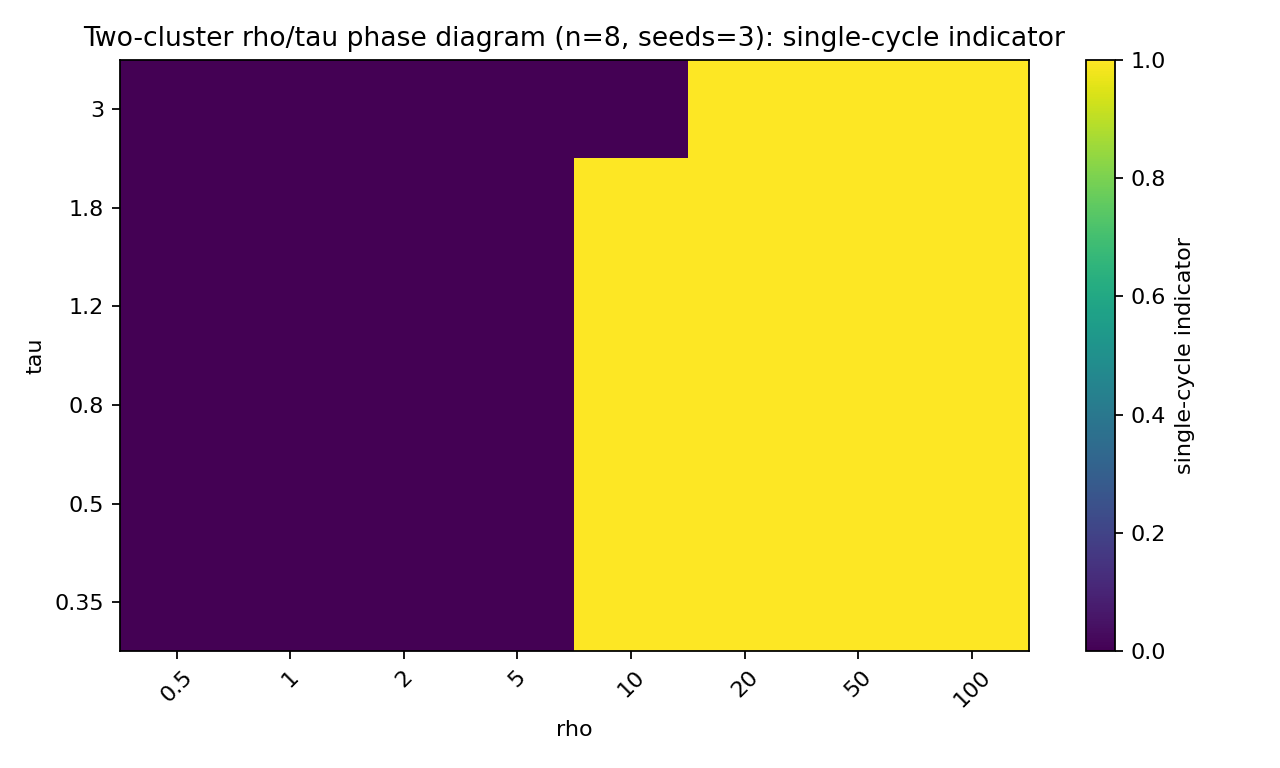
\includegraphics[width=.32\linewidth]{two_cluster_phase_assignment_single_cycle.png}\hfill
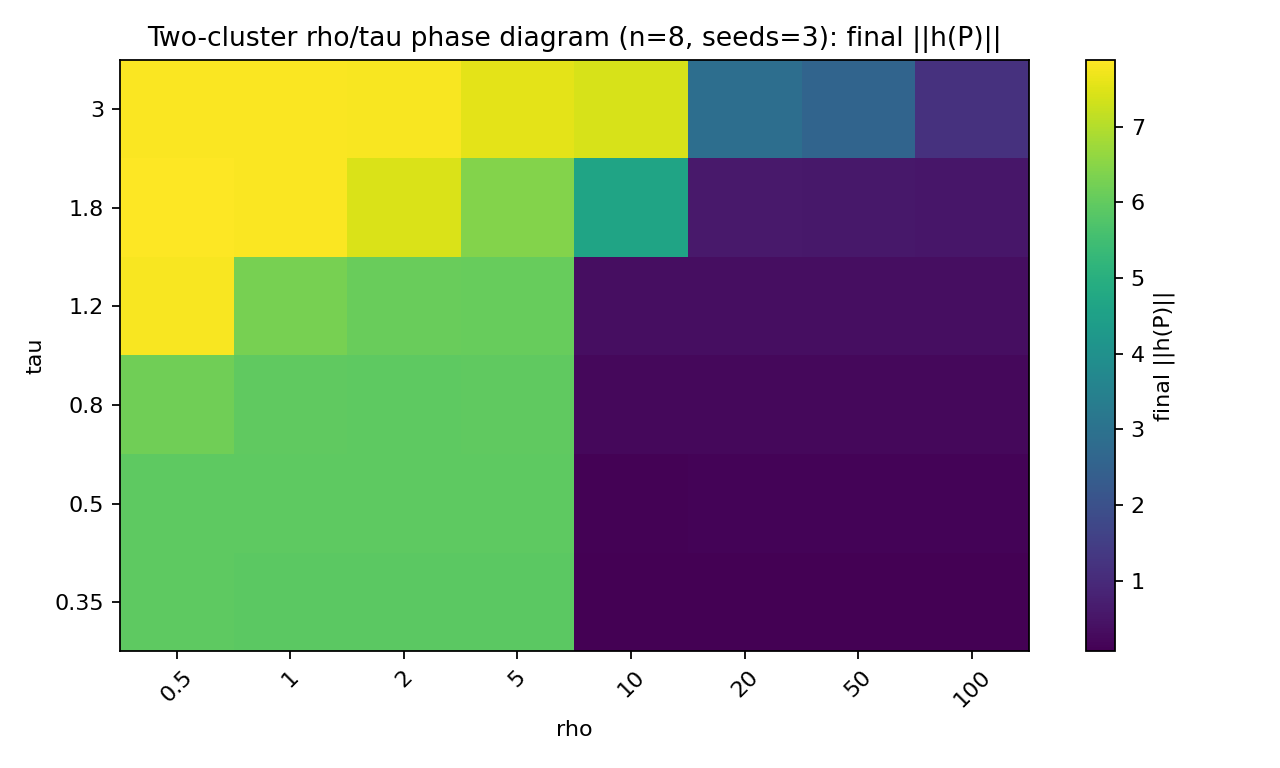
\includegraphics[width=.32\linewidth]{two_cluster_phase_h_norm.png}\hfill
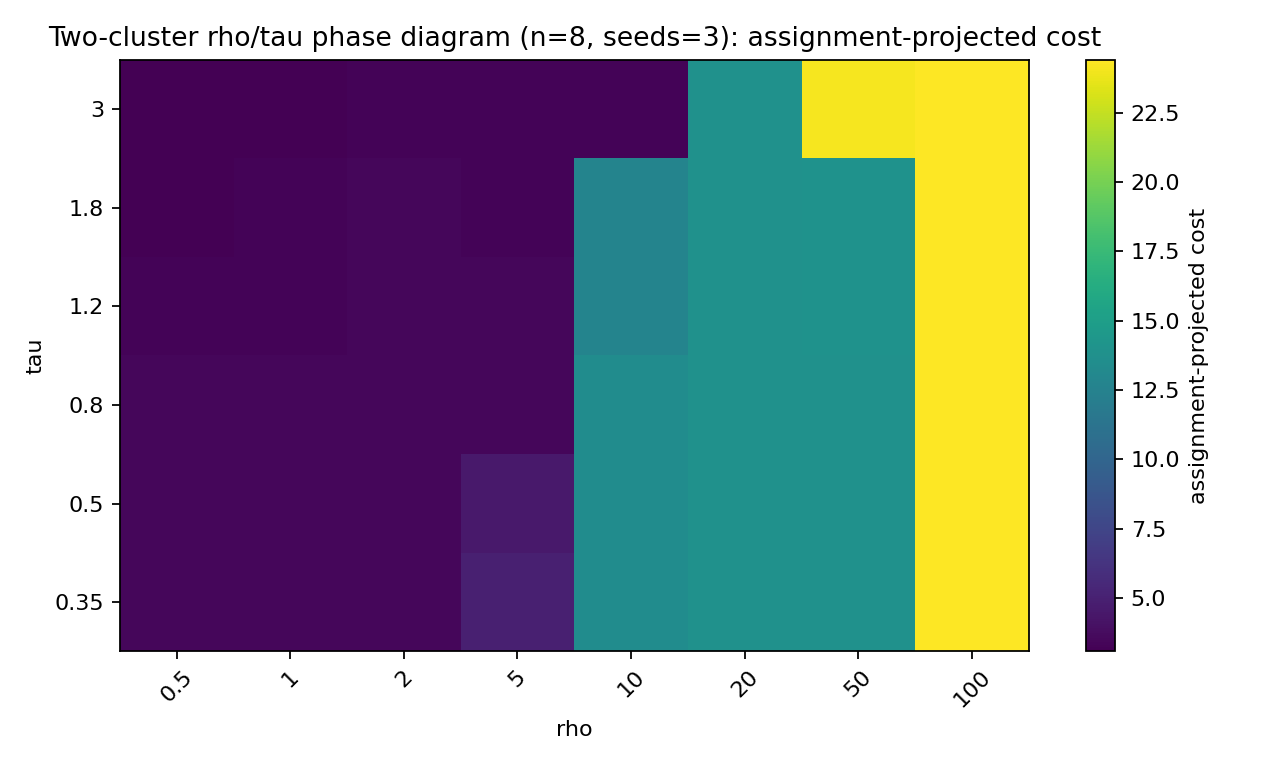
\includegraphics[width=.32\linewidth]{two_cluster_phase_assignment_cost.png}
\caption{Two-cluster phase diagram. Trace pressure controls the transition to single-cycle assignments; assignment cost can rise sharply in the Hamiltonian phase.}
\label{fig:phase-diagram}
\end{figure}

\subsection{Uniform degeneracy and ringing}

The uniform diagnostic confirms first-order trace-gradient collapse at exact uniform initialisation in the no-self-loop setting. The linearised top-mode experiment shows pure primal-dual ringing and augmented damping.

\begin{figure}[ht]
\centering
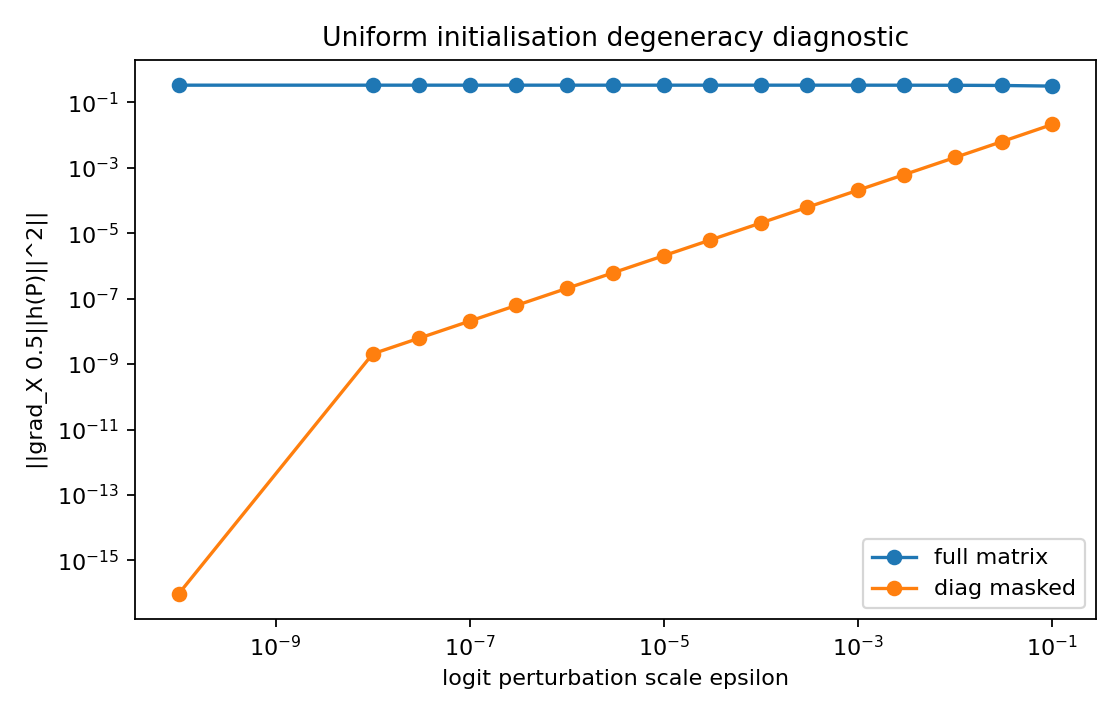
\includegraphics[width=.48\linewidth]{uniform_degeneracy_grad_norm.png}\hfill
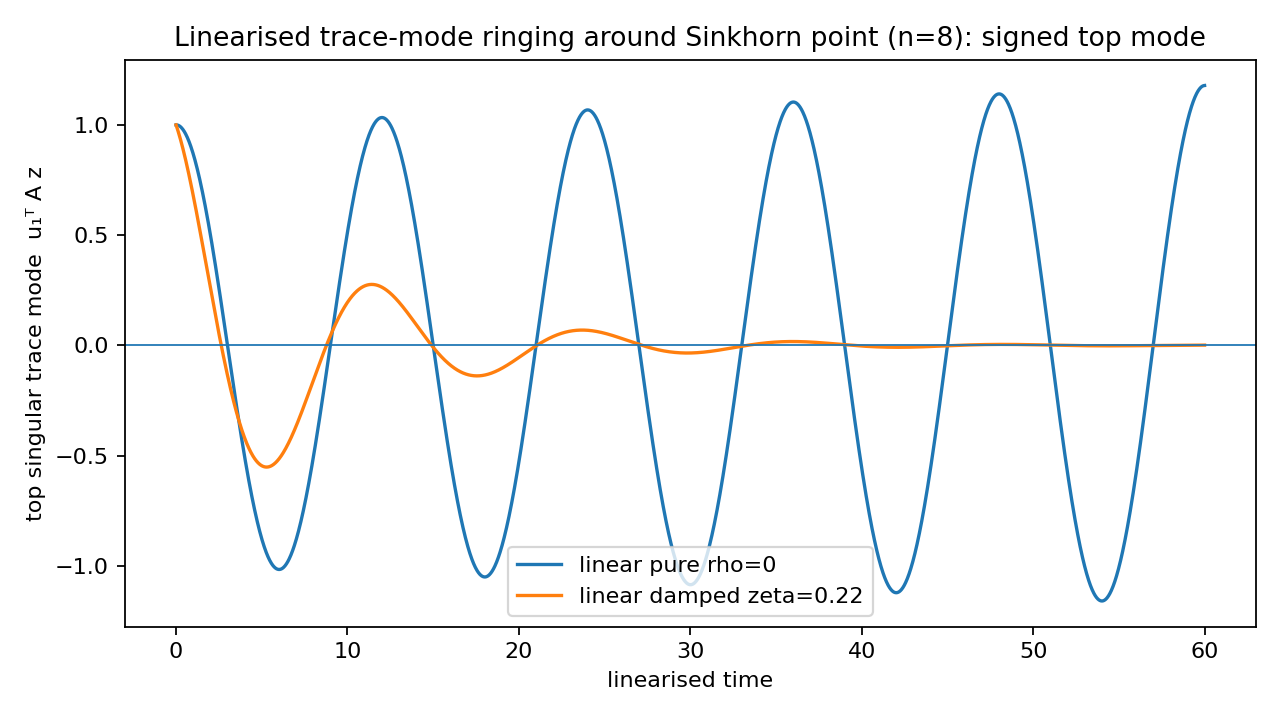
\includegraphics[width=.48\linewidth]{ringing_linear_top_mode.png}
\caption{Left: uniform initialisation degeneracy. Right: linearised top trace mode, showing undamped primal-dual oscillation and augmented damping.}
\label{fig:uniform-ringing}
\end{figure}

\subsection{Nonlinear primal-dual snapping}

In the full nonlinear Sinkhorn/logit system, pure primal-dual dynamics often appears as delayed high-residual plateaus followed by snapping rather than a clean sinusoid. Augmentation damps the trace-visible modes directly.

\begin{figure}[ht]
\centering
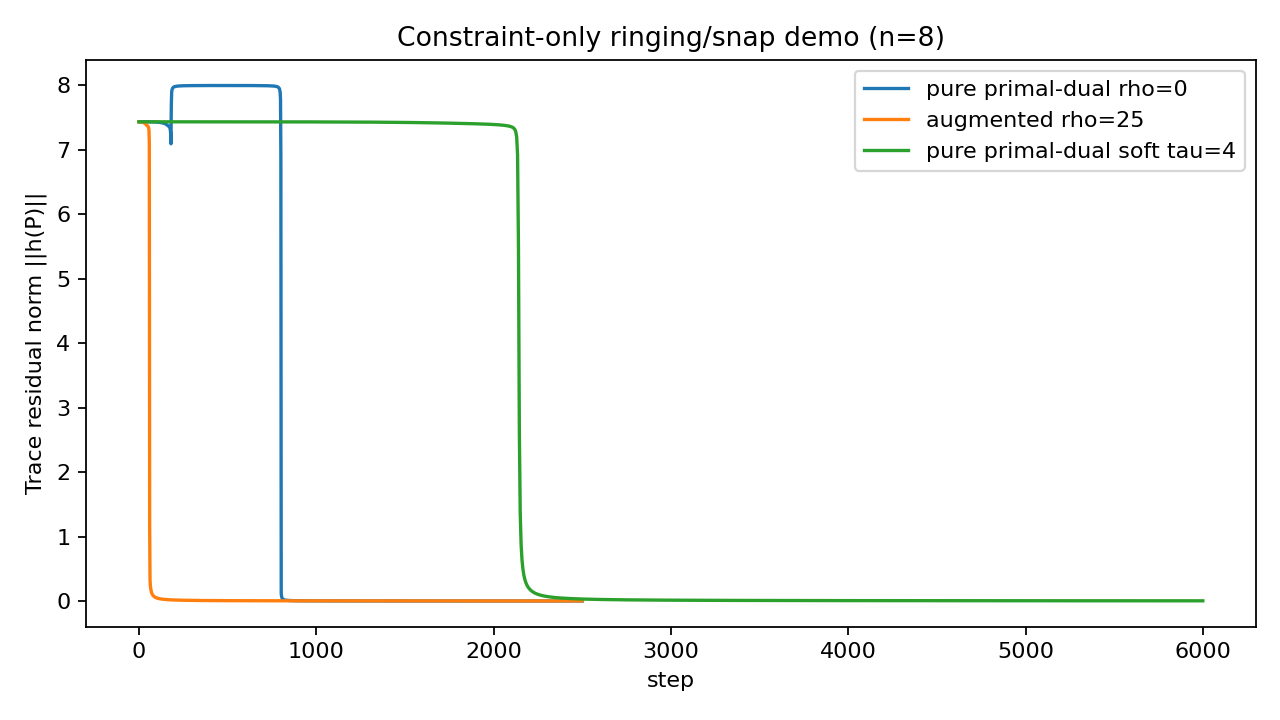
\includegraphics[width=.48\linewidth]{ringing_h_norm.png}\hfill
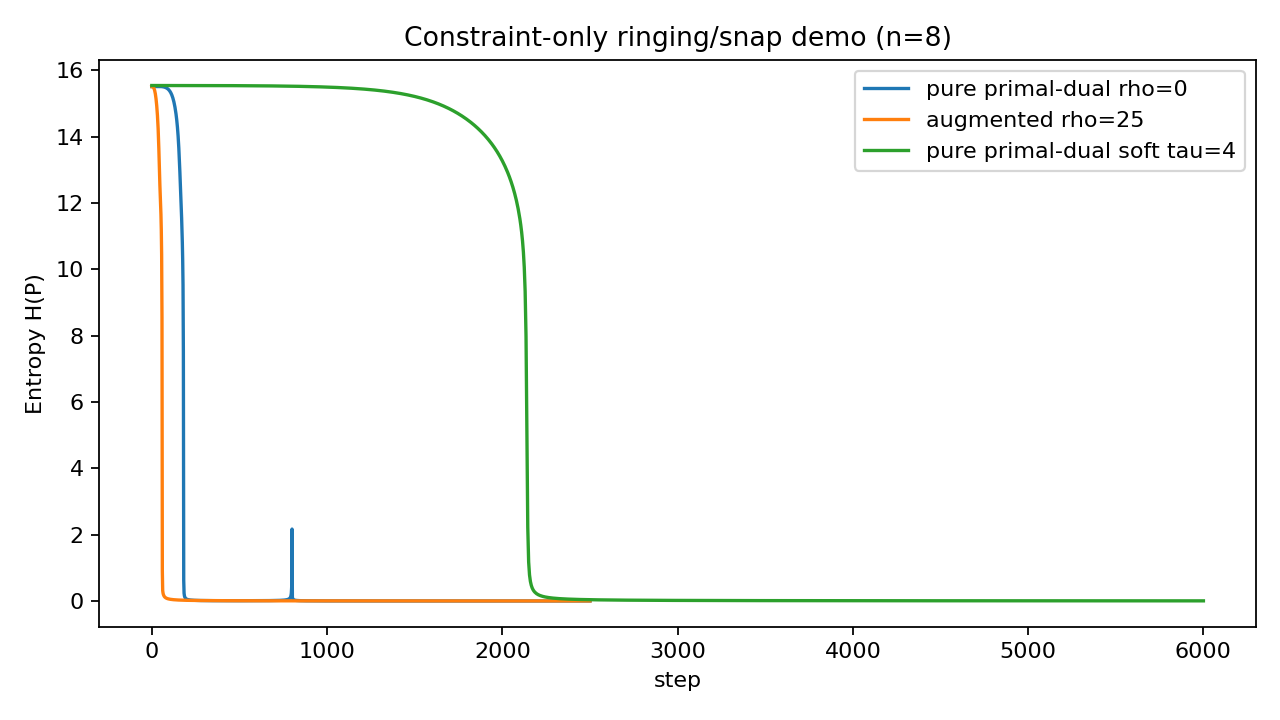
\includegraphics[width=.48\linewidth]{ringing_entropy.png}
\caption{Nonlinear primal-dual diagnostics. The full dynamics can show delayed collapse and support hardening rather than smooth small-signal ringing.}
\label{fig:nonlinear-snap}
\end{figure}

\section{Relation to Brockett flow}

The analogy with Brockett's double-bracket flow is structural rather than literal. Classical Brockett-style flows use orthogonal/isospectral geometry, commutator projection, and sorting/diagonalisation by a potential. The present flow uses Birkhoff/transport-polytope geometry, Sinkhorn/KL projection via row-column potentials, and cycle-moment shaping by a routing cost. In Brockett flow, commutators remove forbidden normal directions on an isospectral orbit. Here, row/column potentials remove forbidden marginal directions on the Birkhoff polytope.

A concise description is: a transport-polytope analogue of Brockett flow, where isospectral commutator geometry is replaced by KL/Sinkhorn geometry, and Hamiltonian cycles arise as trace-moment constrained boundary strata.

\section{Discussion and open questions}

The experiments support the stability analysis rather than a solver-performance claim. The main picture is:
\begin{enumerate}
    \item continuation can recover an obvious geometric tour;
    \item fixed trace pressure can produce valid but poor tours;
    \item clustered instances reveal cheap subtour attractors;
    \item increasing $\rho$ produces a transition from subtours to single cycles;
    \item exact uniform initialisation is first-order degenerate under no-self-loop trace constraints;
    \item linearised primal-dual trace modes ring without augmentation;
    \item augmented penalties damp trace-visible modes.
\end{enumerate}

Open questions include: the best citation lineage for the trace/Hamiltonian characterisation; the exact rank of the trace-constraint Jacobian at symmetric points; adaptive tuning of $\rho$ using the spectrum of $AMA^\top$; a rigorous reduced-cost stability theorem for alternating-cycle exchanges; and extensions to rectangular transport polytopes, partial matchings, capacity-constrained routing, and sparse attention maps.

\bibliographystyle{plainnat}
\bibliography{references}

\end{document}
